% !TeX root = interim.tex

\iffalse


\fi

\subsection{Status Quo}

    The individual milestones of the projects are discussed below briefly in relation to their corresponding aims and objectives from the proposal report \autocite{proposal_report}. Each of the milestones is also discussed in more detail in their respective sections of the report shown in brackets.
    
    \begin{itemize}
        \item \textbf{Simulating the communication channel and transmitter/receiver}
        \\
        So far we have implemented an optical channel model consisting of chromatic dispersion, square-law detection and thermal noise (\S \ref{sec:optical_channel_model}). In addition to this digital signal processing tools such as pulse shaping with different pulse shapes were implemented to simulate pulse amplitude modulation (PAM) signal transmission with efficient bandwidth usage. As well as pulse shaping, helper functions to plot bit-error-rate vs signal-to-noise ratio (BER vs SNR) and eye-diagrams were also implemented (\S \ref{sec:dsp_tools}).
        
        \item \textbf{Choosing an appropriate neural network architecture}
        \\
        The neural network configuration discussed in \autocite{8433895} was also replicated as a starting point for our objectives. Two neural networks have been implemented for the transmitter and receiver integrating the channel model in between (\S \ref{sec:replication_of_e2e_ae}). In order to improve the accuracy of the neural networks, the particle swarm optimisation technique was implemented and resulted in significant improvement in performance over the previous model (\S \ref{sec:application_particle_swarm_optimization}). The selection of the neural network type and training method is still ongoing as different architectures are being considered. Furthermore, the performance of the neural networks on hardware is yet to be seen.
        
        \item \textbf{Implementing the neural network on an FPGA}
        \\
        Research was performed on the choices for FPGA available to us for the hardware implementation (\S \ref{sec:fpga_choice}). Additionally, basic neural networks were implemented in a hardware description language (HDL) (\S \ref{sec:neural_network_hdl}). Finally, neural networks were tested with reduced precision data types to find a compromise between efficiency and accuracy for the hardware implementation (\S \ref{sec:reduced_precision_data_types}).
    \end{itemize}
    
    As for the future of the project, the aims and objectives that will be of primary focus will be finalizing a neural network model that outperforms traditional compensation techniques as well as its hardware implementation. Once the FPGA, analog-digital converter (ADC) and digital-analog converter (DAC) have been ordered, progress can be made on porting the architecture from python to HDL.

\clearpage

\subsection{Project Schedule}

    The updated project timeline in the form of a Gantt chart can be found in \autoref{app:gantt_chart}. So far we have been on track with our initial timeline that was discussed in our project proposal \autocite{proposal_report}. Progress was halted closer to the end of the term due to assignment deadlines for other modules. However we plan to make up the lost time over the Christmas holiday to ensure that we will not fall behind schedule. We plan to have a neural network architecture chosen and implemented in python by the start of the next term in January 2021. Furthermore we also plan to have chosen FPGA, DAC and ADC components for system demonstration by then. This will ensure that the project can progress as planned.

\subsection{Supporting Theory}

    \subsubsection{Neural Networks and Deep Learning}
    \label{sec:neural_network_theory}
    \hspace*{0pt}\hfill \textit{Oliver Jaison}\\
        
        \begin{figure}[H]
            \centering
            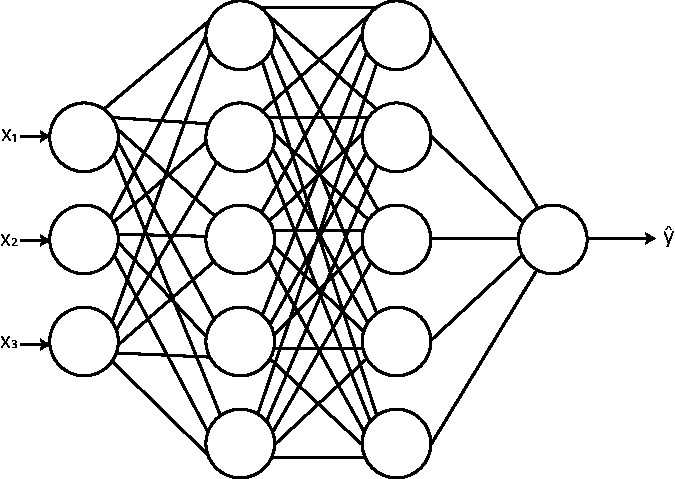
\includegraphics[scale=0.7]{mlp.pdf}
            \caption{A very simple neural network; A fully connected multi-layer perceptron with 2 hidden layers and one output layer. The vector $\boldsymbol{x}$ is the input ($\boldsymbol{x} \in \rm I\!R^{3}$) and $\hat{y}$ is the output}
            \label{fig:simple_neural_network}
        \end{figure}
        
        Neural networks solve problems by learning optimal parameters to map a set input samples onto given output labels. They consist of layers which in turn consist of individual cells called neurons. Each neuron linearly transforms its output and then passes the output through a non-linear function to produce its activation which is its output. A simple neural network is shown in \autoref{fig:simple_neural_network}. Some examples of non-linear activation functions are given in \autoref{eqn:activation_functions}:
        
        \begin{equation}
	    	\label{eqn:activation_functions}
	    	\begin{split}
	    		f_{ReLU}(\boldsymbol{z})_i &= \max(0,z_i) \;\; \text{for} \;\;  i = 1, 2, \dots , K\\
	    		f_{tanh}(\boldsymbol{z})_i &= \frac{e^{z_i}-e^{-z_i}}{e^{z_i}+e^{-z_i}} \;\; \text{for} \;\;  i = 1, 2, \dots , K\\
	    		f_{sigmoid}(\boldsymbol{z})_i &= \frac{1}{1+e^{-z_i}} \;\; \text{for} \;\;  i = 1, 2, \dots , K\\
	    		f_{sigmoid}(\boldsymbol{z})_i &= \frac{1}{1+e^{-z_i}} \;\; \text{for} \;\;  i = 1, 2, \dots , K\\
	    		f_{leakyReLU}(\boldsymbol{z})_i &= 
                \begin{cases}
                    0.001z_i \quad & \text{if $z_i\leq 0$} \\
                    z_i \quad & \text{if $z_i>0$}
                \end{cases}
                 \;\; \text{for} \;\;  i = 1, 2, \dots , K\\
	    		f_{softmax}(\boldsymbol{z})_i &= \frac{e^{z_i}}{\sum_{j=1}^{K}e^{z_j}} \;\; \text{for} \;\;  i = 1, 2, \dots , K
	    	\end{split}
	    \end{equation}
        where $\boldsymbol{z} \in \mathbb{R}^K$ is the output of the layer.
        \\
        
        Autoencoders are a special type of neural network where, rather than the number of neurons increasing in subsequent hidden layers from the input layer, we impose a bottleneck. This means that the number of neurons is lower than the number of inputs in the input layer. This results in a compressed representation of the input data. Traditionally this is an unsupervised learning algorithm but it is made semi-supervised by comparing the output of the autoencoder to the input and minimising the error between them.
        \\
        
        \autocite{8820761} explains that autoencoder based compression methods in communication channels learn the statistical regularities in the data. This could be key in an error correcting system for a transmitter receiver pair with correlated input data.
        \\
        
        \autoref{fig:autoencoder} shows a very basic autoencoder but similarly with neural networks you can have different categories of autoencoder. \autocite{9058605} discusses a de-noising autoencoder. A de-noising autoencoder will corrupt the input on purpose then compare the output to the un-corrupted input to generate a loss function. This loss function is then fed back into the input to make the network robust against the particular kind of noise it was trained against.
        \\
        
        \cite{7836672} discusses using these de-noising techniques for medical images against Gaussian and Poisson noise. It can be seen that even with a small data set, good performance is achieved, even with a noisy image type.
        \\
        
        \begin{figure}[H]
            \centering
            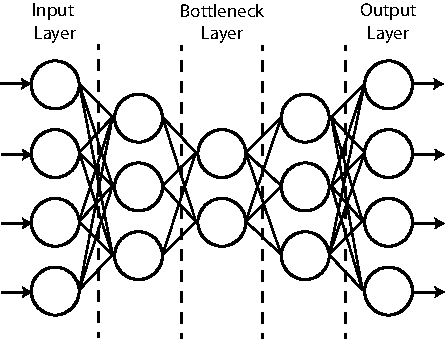
\includegraphics[scale=1.3]{simple_autoencoder.pdf}
            \caption{Diagram representing a very basic autoencoder. It can be seen the the hidden layers introduces fewer and fewer nodes from the input layer. In doing so creates a bottle neck for the input data.}
            \label{fig:autoencoder}
        \end{figure}
        
    \subsubsection{Particle Swarm Optimisation}
    \label{sec:particle_swarm_optimization_theory}
    \hspace*{0pt}\hfill \textit{An Vo}\\
    
        Particle swarm optimisation (PSO) is an algorithm developed by J. Kennedy and R. Eberhart \autocite{488968} that is used to optimise nonlinear continuous functions, inspired by the concept of swarm intelligence such as in bird flocking and schooling in nature. It involves the use of a population (swarm) of candidate solutions (particles) which move around in a search space. Through an iterative process, the swarm searches for new locations of each particle by its velocity term which optimises based on the global best and their own best. The velocity V and position P of each particle can be defined in these equations:
        
        \begin{equation}
            \label{eqn:pso_equation}
            V_i(t+1) = \omega V_i(t) + c_1r_1(pbest(i,t) - P_i(t)) + c_2r_2(gbest(t) - P_i(t))
        \end{equation}
        \begin{equation}
            \label{eqn:pso_equation}
            P_i(t+1) = P_i(t) + V_i(t+1)
        \end{equation}
        
        where $\omega$ is the inertia weight used to balance the global and local learning rates, r\textsubscript1 and r\textsubscript2 are random variables in range of 0 to 1, c\textsubscript1 and c\textsubscript2 are positive constant parameters known as acceleration coefficients \autocite{PSO_paper}. These velocity and position vectors are the equivalent of weights and biases in a conventional neural network.
        \\
        \\
        This algorithm has been shown to have the application of optimising feedforward neural networks \autocite{884366}. Both the architecture and the weights of a neural network can be adjusted in order to find a version of the neural network that provides the best quality performances. Due to the nature of PSO, there are no selection and crossover operators and each individual particle in the current population has a corresponding particle in the new population. This allows the system to avoid detecting local minimas, preventing premature convergence.
        
    \subsubsection{Distortions and Noise in Optical Communication System}
    \label{sec:optical_channel_distortions_theory}
    \hspace*{0pt}\hfill \textit{An Vo}\\
        
        An optical communication channel is comprised of a transmitter, receiver and the optical fibre connecting the two together. In order to simulate this communication channel, the mathematical representation of the signal at each stage of the channel needs to be established. The signal that enters the optical fibre is described by its electrical field of the EM field, known as its optical field and is expressed mathematically in the time domain as: 
    
        \begin{equation}
            \label{eqn:optical_field_time}
            A(t, z) = |A(t,z)|e^{j\phi(t,z)}
        \end{equation}
        where $z$ is the distance along the fibre and $t$ is the time. $A(t,z)$ is a phasor incorporating the optical amplitude $|A(t,z)|$ and optical phase $\phi(t,z)$.
        \\
        
        The signal suffers from chromatic dispersion as it traverses through the optical fibre, resulting in different frequency components of the signal being delayed by different amounts. For simulation simplicity, this effect will be simulated in the frequency domain due to a linear time delay vs frequency and can be expressed by the following mathematical expression:
        
        \begin{equation}
            \label{eqn:optical_field_freq}
            A(\omega,L) = A(\omega,0)e^{j\frac{1}{2}\beta_z\omega^2L}
        \end{equation}
        where $\omega$ is angular frequency, $\beta_z$ is the group velocity dispersion and $L$ is the fibre length.
        \\
        
        At the receiver, photo-detection is carried out by using the proportional relationship between the output voltage and power of the signal which in turn is proportional to the square of the magnitude of the optical field, resulting in the following mathematical expression.
        
        \begin{equation}
            \label{eqn:squared_law_detection}
            V_{out}(t) = |A(t,L)|^2
        \end{equation}
        where $A(t,L)$ is the inverse Fourier transform of \autoref{eqn:optical_field_freq}.
        \\
        
        To complete the mathematical representation of the signal through an optical channel, the receiver noise is applied to the photo-detected signal. This is in the form of white Gaussian noise (randomly generated voltages $\Delta V(t)$, which are generated with a normal distribution) which is added to both the model shot noise and the thermal noise. This voltage waveform is then the representation of the signal after it leaves the receiver.
        \\
        
        The transmitting and receiving end as well as the channel itself were simulated as a channel model. The neural networks will most likely be implemented using the TensorFlow package with python. The python programming language was chosen for quick prototyping purposes as well as compatibility with TensorFlow. TensorFlow allows for quick experimentation and configuration of different neural network architectures. The above proposed model would be treated as a black box between the transmitting and receiving neural network. 
    
\subsection{Progress to Date}
\label{sec:progress_to_date}

    \subsubsection{Familiarization with TensorFlow}
    \label{sec:familiarization_tensorflow}
    \hspace*{0pt}\hfill \textit{Tharmetharan Balendran}\\
    
        As a starting point we sub-classed from the \texttt{tensorflow.keras.Model} class to create a custom autoencoder model. Two sequential models were implemented: one for the encoder and one for the decoder, and their corresponding layers were added. The input was one-hot encoded, resulting in a vector of size $m=2^N$ where $N$ is the number of bits encoded per message. The following fully connected dense layers were of size $2m$, each followed finally by an output layer of size 2 corresponding to an in-phase (I) output and a quadrature (Q) output. Both of these outputs pass through a channel model. Initially in simulation, this model was taken to be a simple additive white Gaussian noise (AWGN) model. The decoder is symmetrical to the encoder with an input layer of size 2 followed by two fully connected dense layers of size $2m$ each. Finally a output softmax layer of size $m$ produces a vector of probabilities. The full architecture is also represented in the diagram shown in \autoref{fig:iq_autoencoder_diagram}.
        \\
        
        It should be noted that this implementation of the autoencoder produces IQ outputs which is incompatible with intensity modulation direct detection (IM-DD) optical modulation schemes. Therefore, this model was primarily used for familiarization with the TensorFlow package as well as quick prototyping of different approaches. The autoencoder model described in \S \ref{sec:replication_of_e2e_ae} was designed to be compatible with IM-DD modulation schemes.
    
        \begin{figure}[H]
    		\centering
    		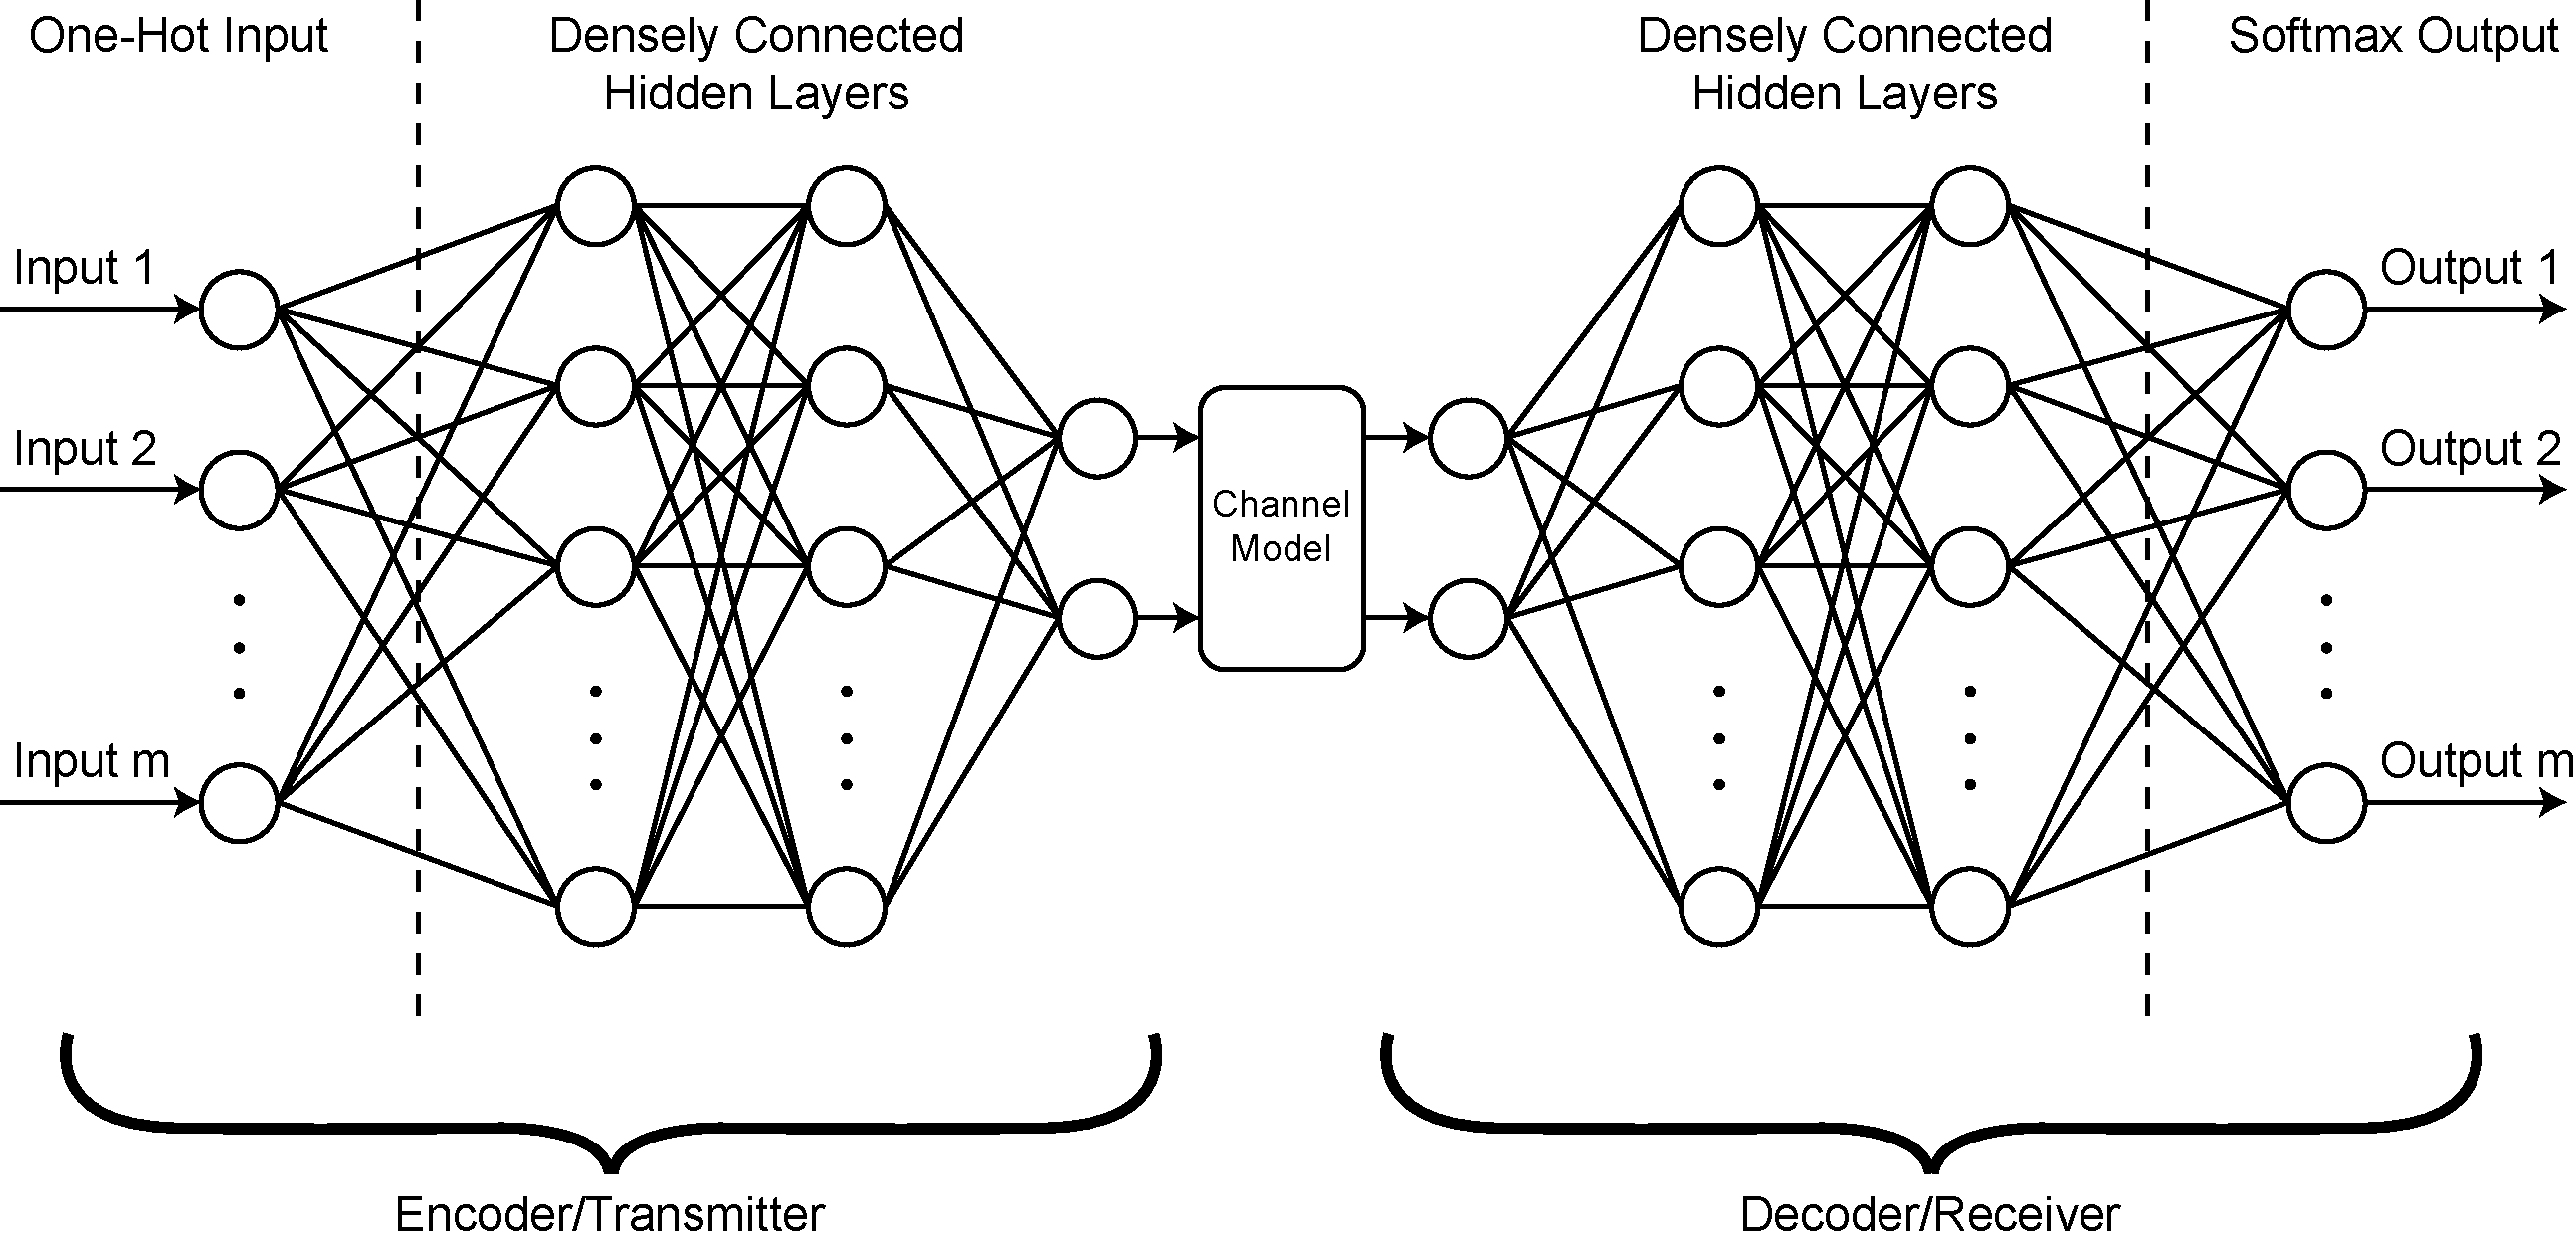
\includegraphics[scale=0.35]{iq_autoencoder_diagram.pdf}
    		\caption{Diagram representing the neural network that was implemented. The encoding and decoding sections are also labelled. The one-hot input layer is of size $m=2^N$ where $N$ is the number of bits encoded per message. The softmax output layer produces a probability vector conveying the probability that the received signal corresponds to any of the messages.}
    		\label{fig:iq_autoencoder_diagram}	
    	\end{figure}
    
    \subsubsection{Optical Channel Model}
    \label{sec:optical_channel_model}
    \hspace*{0pt}\hfill \textit{Tharmetharan Balendran}\\
    
        The optical channel model consists of three main components: The application of chromatic dispersion, the square-law detection as well as the addition of Gaussian noise. The chromatic dispersion was applied by taking the fast Fourier transform (FFT) of the incoming signal and applying a phase shift that is proportional to the frequency as shown by \autoref{eqn:optical_field_freq}. Following this, the signal is transformed back to time domain using an inverse fast Fourier transform (IFFT). After the chromatic dispersion is applied, the detection of the signal by a photodiode is simulated. This is represented by \autoref{eqn:squared_law_detection}. The absolute value of the signal is taken and squared to produce the receiver output. Following this, AWGN was applied to simulate noise arising from the receiver components (amplifiers, thermal noise, etc.) The figures in \autoref{fig:optical_channel_model_signals} show the distortion being applied for a simple on off keying (OOK) modulation scheme with rectangular pulse shapes. 
        
        \begin{figure}[H]
    		\begin{subfigure}{0.5\textwidth}
    			\centering
    			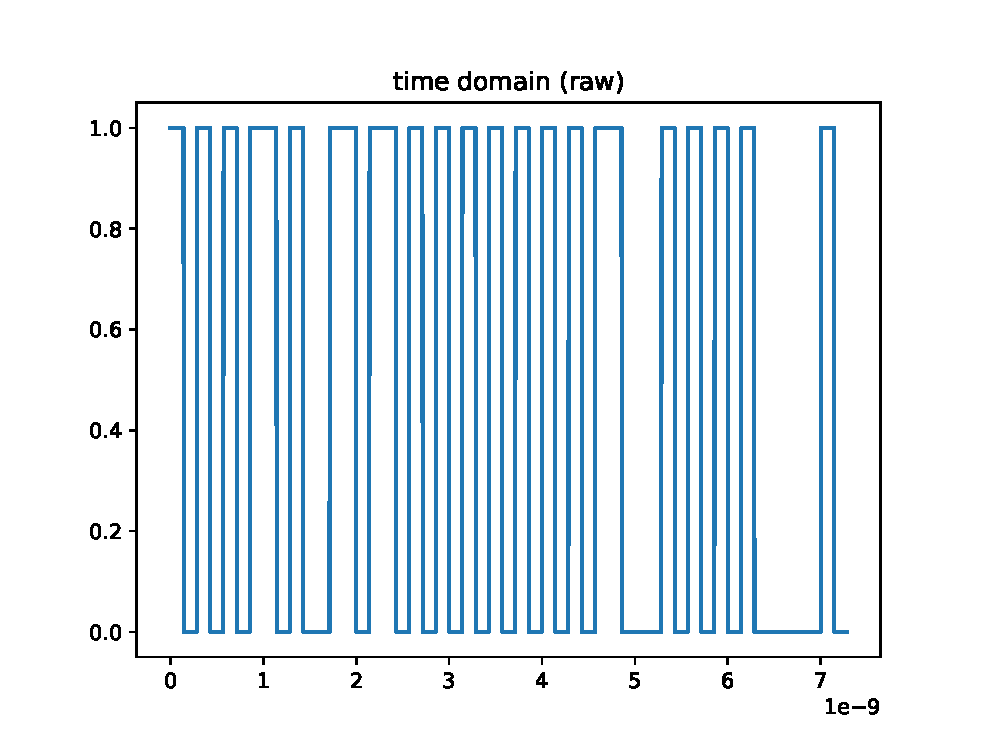
\includegraphics[width=\textwidth]{transmitted_signal.eps}
    			\caption{Transmitted signal using a OOK modulation for simplicity.}
    			\label{fig:transmitted_signal}	
    		\end{subfigure}
    		\begin{subfigure}{0.5\textwidth}
    			\centering
    			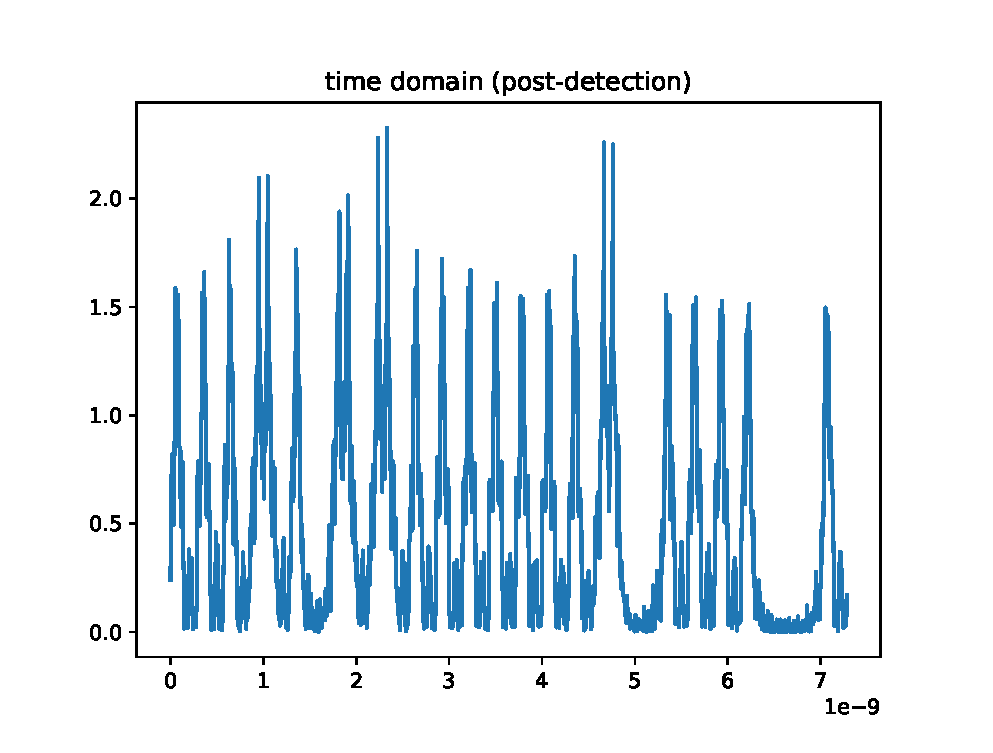
\includegraphics[width=\textwidth]{signal_post_detection.eps}
    			\caption{Received signal after all distortions of the signal have been applied.}
    			\label{fig:signal_post_detection}	
    		\end{subfigure}
    		\caption{Plots showing the distortion of the transmitted signal over an optical fibre of length 50km with a group velocity dispersion of -21.7 $ps^2/km$. The sample rate was set to 336 GHz while the bit rate was set to 7 Gbit/s}
    		\label{fig:optical_channel_model_signals}
    	\end{figure}
    
    \subsubsection{Implementation of DSP and Signal Analysis Techniques}
    \label{sec:dsp_tools}
    
        \textbf{Pulse Shaping} \hspace*{0pt}\hfill \textit{Tharmetharan Balendran}\\
        
            Different pulse shapes were implemented to enable the transmission of PAM signals with efficient bandwidth usage. The pulse shapes to choose from in the simulation are: rectangular, raised cosine and root raised cosine. These were implemented by convolving their impulse functions with the time domain representation of the signal. The raised cosine filter pulse shape can be seen in the eye diagram in \autoref{fig:eye_diagram}. The matched filters corresponding to the pulse shapes was also implemented. However in the optical channel, due to the square-law detection, the signal gets distorted and the matched filter sampling results in a sub-optimal BER.
            \\
        
        \textbf{BER vs SNR} \hspace*{0pt}\hfill \textit{Oliver Jaison}\\
        
            To quantify the performance of the system, code was written to generate a graph of BER vs SNR as shown in \autoref{fig:autoenc_quant}. This way we could measure the performance of the model and the channel.
            \\
            
        \textbf{Eye Diagrams} \hspace*{0pt}\hfill \textit{Oliver Jaison}\\
        
            Upon observing unexpected results from the BER vs SNR figures we implemented code to generate an eye diagram for the transmitted signal so that the quality of the signal could be analysed. An example of this can be seen in \autoref{fig:eye_diagram}.
        
        \begin{figure}[H]
    		\begin{subfigure}{0.5\textwidth}
    			\centering
    			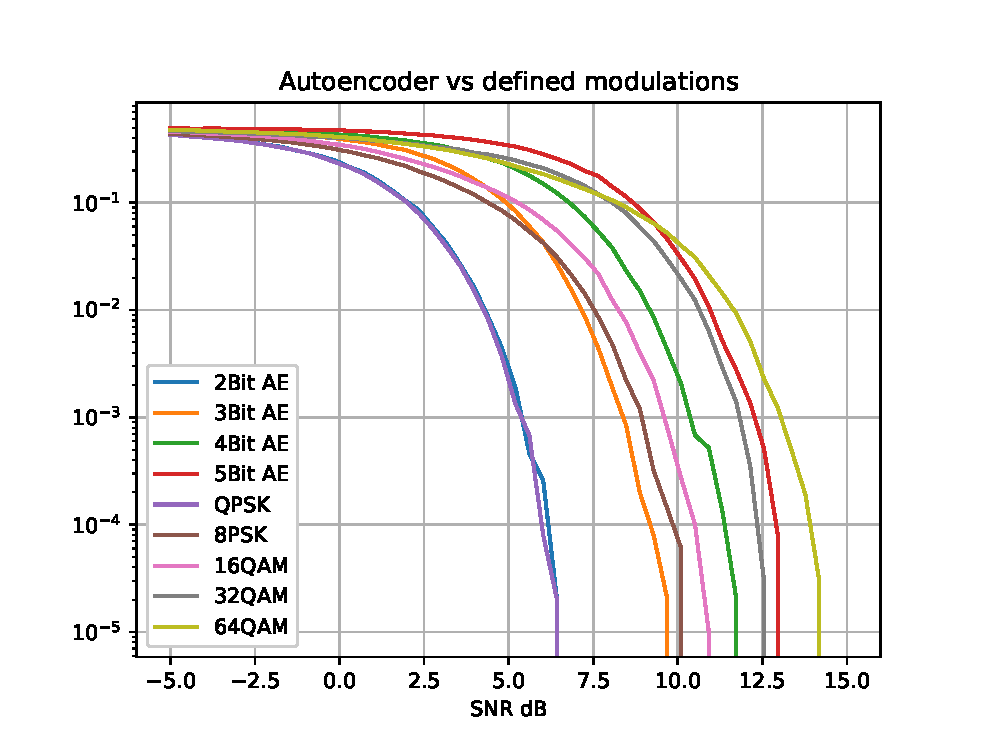
\includegraphics[width=1.1\textwidth]{autoencoder_mods.eps}
    			\caption{This figure shows a graph of BER against SNR for different modulation methods.}
    			\label{fig:ber_vs_snr}	
    		\end{subfigure}
    		\begin{subfigure}{0.5\textwidth}
    			\centering
    			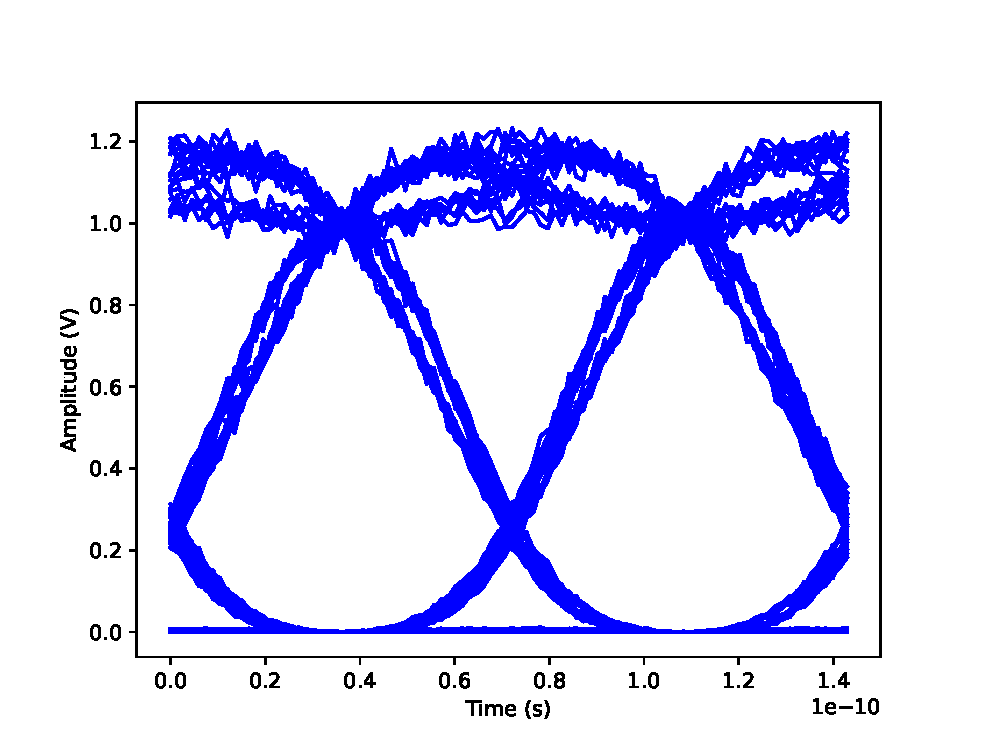
\includegraphics[width=1.1\textwidth]{eye_diagram.eps}
    			\caption{This is an example eye diagram of a received signal of a 2PAM modulated signal with a raised cosine pulse shape.}
    			\label{fig:eye_diagram}	
    		\end{subfigure}
    		\caption{Plots of different performance measuring metrics used to identify any faults in the channel models or modulation techniques.}
    		\label{fig:optical_channel_model_signals}
    	\end{figure}
    
    \subsubsection{Replication of Neural Network discussed by Karanov et al. \autocite{8433895}}
    \label{sec:replication_of_e2e_ae}
    \hspace*{0pt}\hfill \textit{Tharmetharan Balendran}\\
    
        The neural network configuration discussed in the paper by Karanov et al. demonstrated promising results and was chosen as a good stating point. The paper discussed a simple feed-forward neural network autoencoder. The encoding neural network acts as a modulator and produces encoded symbols for each message at the bottleneck layer. The bottleneck output is passed through a channel model to simulate transmission distortions and then passed into the decoding neural network that acts as the demodulator. On the encoding neural network, $N$ identical neural networks encode $N$ consecutive messages into $N$ consecutive symbols each consisting of $n$ samples. These symbols are then serialized to form a single stream of $n\times N$ samples. This ensures that inter-symbol interference (ISI) can be modelled by considering neighbouring symbols. At the decoding neural network, the central symbol is extracted and demodulated. The complete architecture of the autoencoder can be seen in \autoref{fig:end_to_end_autoencoder_diagram}.
        
        \begin{figure}[H]
    		\centering
    		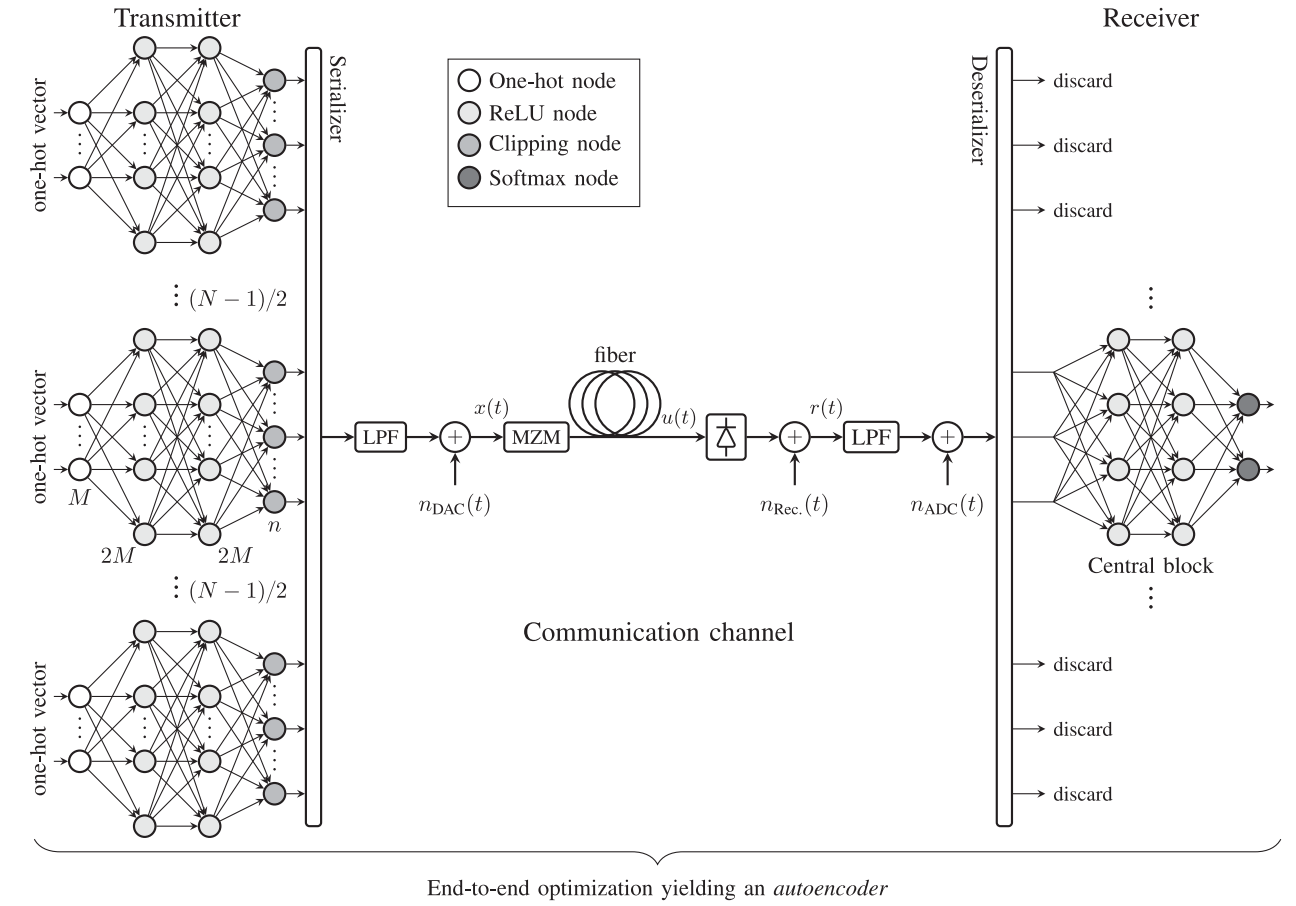
\includegraphics[width=0.9\textwidth]{end_to_end_autoencoder_diagram.png}
    		\caption{The diagram taken from \autocite{8433895} depicting the overall configuration to enable learning of symbols.}
    		\label{fig:end_to_end_autoencoder_diagram}	
    	\end{figure}
        
        A similar implementation of the autoencoder was configured using the TensorFlow package in python. In this implementation the simulation of the Mach-Zehnder modulator (MZM) was left out to simplify the channel model. As the MZM operates linearly for small amplitudes, this assumption would not harm the accuracy of the simulation greatly. To enable this, the optical channel model had to be re-developed to be compatible with TensorFlow's tensor datatype. This was achieved by utilizing TensorFlow functions for FFT as well as tensor multiplication. The optical channel was implemented as a TensorFlow layer and can therefore be placed in-between the encoder and decoder.
        \\
    
        Symbol mapping similar to those discussed in \autocite{8433895} was achieved. A complete mapping of messages onto symbols can be seen in \autoref{app:learnt_symbol_mapping}. No specific mapping of bits onto symbols was enforced meaning that no assessment as to the potential BER of the system can be made. From testing the autoencoder with appropriate noise a symbol error rate of around $1\times10^{-2}$ was observed. The simulation parameters are given in \autoref{tab:simulation_parameters}.
        \\
        \begin{table}[H]
            \centering
            \begin{tabular}{ll}
                \textbf{Parameter}                              & \textbf{Value}            \\ \hline
                Sampling Frequency ($f_{s}$)                    & $336\;GHz$                 \\
                Message Cardinality ($M$)                       & $32$                      \\
                Samples per Symbol ($n$)                        & $24$                      \\
                Messages per Block ($N$)                        & $9$                       \\
                Dispersion Factor ($\beta$)                     & $-21.7\;ps^{2}km^{-1}$     \\
                Fiber Length ($L$)                              & $50\;km$                   \\
                Receiver Noise stddev ($\sigma_{rx}$)            & $0.01$                    \\
                Quantization Noise stddev ($\sigma_{q}$)        & $0.002$
            \end{tabular}
            \caption{Table of simulation parameters used when learning symbol mapping using the end-to-end autoencoder.}
            \label{tab:simulation_parameters}
        \end{table}
        
        As the chromatic dispersion results in ISI, an encoder/decoder that is able to consider previously received/transmitted symbols should outperform one that solely considers one symbol at a time. To simulate this, long-short-term-memory (LSTM) layers were implemented at the transmitting and receiving neural networks. These will still need further tuning to produce acceptable results but should outperform the feed-forward neural network architecture.
    
    \subsubsection{Application of Particle Swarm Optimisation} \hspace*{0pt}\hfill \textit{An Vo}\\
    \label{sec:application_particle_swarm_optimization}
        During the initial implementation of a neural network for the autoencoders of the project, there was an issue in which the neural network would detect and converge towards local minima generated by noise in the signal. These lead to the accuracy of the network falling below 50\%. 
        \begin{figure}[H]
        \begin{subfigure}[h]{0.53\linewidth}
        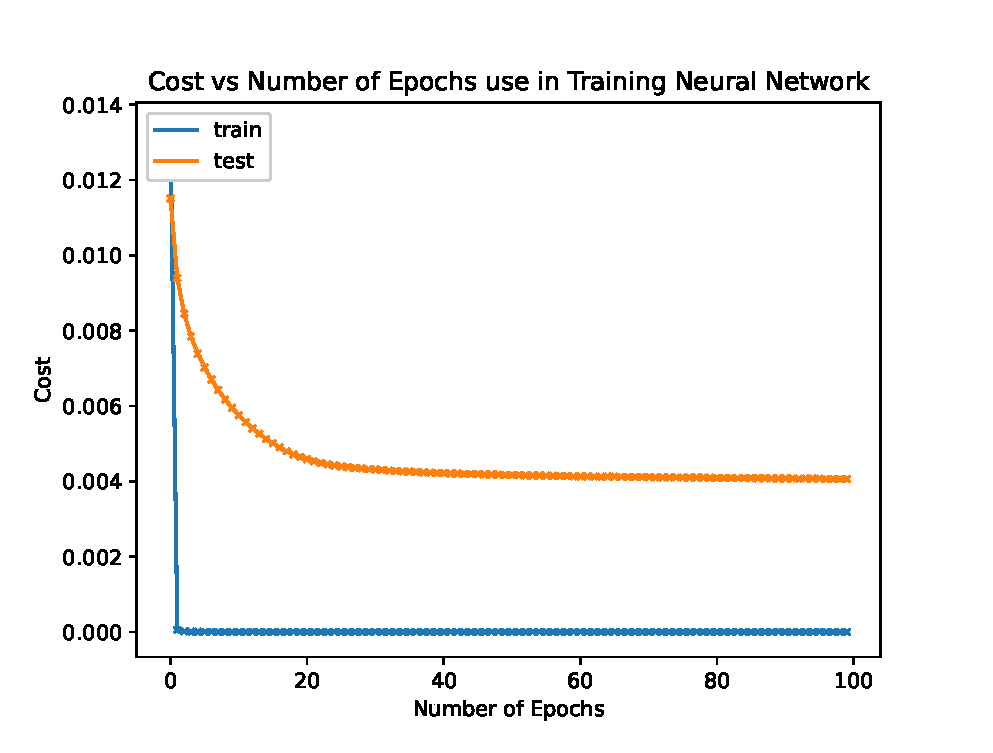
\includegraphics[width=\linewidth]{cost_vs_epoch_NN.eps}
        \caption{Traditional Neural Network}
        \end{subfigure}
        \hfill
        \begin{subfigure}[h]{0.53\linewidth}
        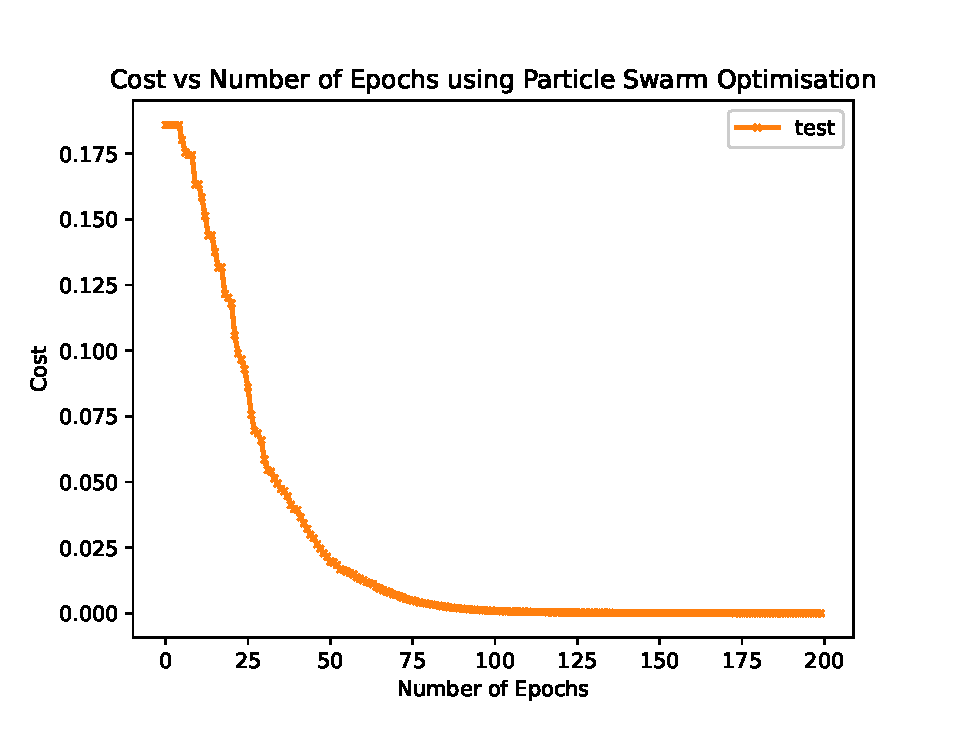
\includegraphics[width=\linewidth]{cost_vs_epoch_PSO.eps}
        \caption{Particle Swarm Optimised Neural Network}
        \end{subfigure}%
        \caption{Learning Curve graphs showing how the number of epochs impacts the cost function}
        \label{fig:cost_functions}
        \end{figure}
        \\
        
        A new system based on the particle swarm optimisation method was implemented using a python library called pyswarms \autocite{pyswarms} using the same neural network architecture and initial weights of the current under-performing network. The implemented PSO model used 100 particles in the swarm with c\textsubscript1 set to 0.5 and c\textsubscript2 set to 0.3. This PSO enabled neural network performed significantly better than the previous model as can be seen from the learning curves in fig \ref{fig:cost_functions}, where the cost of the PSO model converges towards 0 while for the initial neural network, it gets trapped at a local minima preventing the network from learning further.
        \\
        \\
        It was decided that this particle swarm model can be implemented into the finalised autoencoder system as a means to optimise the performance of the applied neural networks for the encoder and decoder.
    \subsubsection{Neural Network Hyperparameter Optimisation}
    \hspace*{0pt}\hfill \textit{An Vo}\\
    \label{sec:neural_network_hyperparameter_optimisation}
        Initially the neural network implemented had a simple architecture of a fully connected network, with a number of densely populated hidden layers which ultimately led to poor performance. Different techniques were applied to improve this model such as batch normalisation between the layers that standardise the inputs to a layer with the effect of stabilising the learning process, and helping the neural network from converging towards a local minima. Dropout layers are added which randomly eliminate some connections between layers, breaking up the fully connected network and helping to prevent overfitting of the training data. Different activation functions such as the rectified linear unit (ReLU), sigmoid and softmax, as well as introducing kernel constraints to limit the change in the magnitude of the weights between epochs were tested.
        \\
        
        Additionally, a grid search technique for model hyperparameter optimisation can be used to further tune the hyperparameters of the network, and involves the manual process of constructing and evaluating model for each combination of parameters provided and cross validating performances for each. This became a very computational taxing task and will require access to more computational power in the form of access to GPU farms. This technique along with the PSO methodology will work to optimise the autoencoder's neural networks.

    \subsubsection{Choice of FPGA, ADC and DAC for Hardware Implementation}
    \label{sec:fpga_choice}
    \hspace*{0pt}\hfill \textit{Mindaugas Jarmolovi\v{c}ius}\\
    
    A number of different options of FPGAs have been considered for implementation of the neural network autoencoder to achieve high throughput transmission on an optical channel. For this an FPGA board (or two boards, one for encoder and one for decoder), ADC and DAC need to be selected.
    \\
    
    To achieve maximum transfer rate in real-time a high performance ADC/DAC were investigated with performance of 3-12 Giga-Samples Per Second (GSPS). Development boards with both an integrated FPGA and a sufficiently high performant ADC/DAC do not exist, therefore different ADC/DAC FPGA Mezzanine Cards (FMCs) were investigated. A list of FMCs are shown in \autoref{table:hw_list}. Note that boards with Parallel LVDS has built-in FPGAs.  Three configurations are available: separate ADC and DAC modules with a single FPGA board with two FMC connectors or two FPGA boards with one connector each; or using a single FMC that integrates both DAC and ADC. Interface is also important because it may cause a bottleneck. Available options are FMC (Vita 57.1) connection capable of datarates of up to 10Gbps (it also has High Pin Count (HPC) and Low Pin Count (LPC) variations); FMC+ (Vita 57.4) connection that allows datarate of up to 28Gbps. Connectors also have a datarate limit that is defined by which and how many FPGA transceivers the FMC interface is physically connected to. Note that FPGA boards with FMC+ connector are compatible with FMC (Vita 57.1) boards but not the other way around. In addition, most of the FMC manufacturers release their own HDL Core that allows for quick implementation, however it is usually developed for a specific FPGA or FPGA board in mind, therefore additional check is also required to find how difficult it is to utilize a particular ADC/DAC with a particular FPGA. 
    
    FPGA selection also depends on multiple additional factors:
    \begin{itemize}
        \item \textit{Number of configurable logic blocks or Look-Up Tables (LUTs)} - needs to be sufficient to support all logic in the neural network.
        \item \textit{Number of Digital Signal Processing (DSP) blocks} - these blocks have built-in floating-point arithmetic units that are faster than ones implemented with LUTs. 
        \item \textit{Memory Technology} - needs to be sufficient to buffer high throughput received data for further BER check. Also, depending on implemented structure, neural network weight and bias values will be stored in memory requiring additional bandwidth for fast operation. DDR3-1866 memory with bandwidth of 14.933GBps might be sufficient for application, especially when using multiple memory channels.
        \item \textit{Transceiver Technology} - used by FMC and is important for sufficient data-rate.
    \end{itemize}
    A number of considered FPGA boards are listed in \autoref{table:fpga_list}. Due to all different parameters and high equipment cost, each configuration should be manually checked in great detail to ensure compatibility. Following configurations are considered:
    
    \begin{itemize}
        \item \textit{ZCU102 FPGA, ADC12DL3200EVM ADC and AD9164-FMCC-EBZ DAC} - this ADC is the fastest board that uses FMC (Vita 57.4) interface. ZCU102 is the one of the most optimal high performance FPGA boards with two FMC connections. DAC is also the most optimal board for a given price. 
        \item \textit{ADS8-V1EBZ FPGA and AD9082-FMCA-EBZ ADC-DAC board} - this ADC\&DAC manual only has implementation documentation on ADS9-V2EBZ FPGA board, therefore a further investigation is needed to check compatibility.
        \item \textit{ZCU104 and AFE7422EVM ADC-DAC board} - Lower price combination with optimal performance. ADC\&DAC board runs up to 15Gbps whereas ZCU104 FMC connector has only single GTH transceiver lane which should be capable in operating up to 16.3Gbps. However, these datarates seems to be outside specification of FMC interface.
    \end{itemize}
    Note that ADC boards with Parallel LVDS and builtin FPGA were not explored in depth. Furthermore, it would be also cost efficient to use ADC08DJ3200EVM ADC board which is high speed of 6.4GSPS and low price due to 8bit precision. However it uses FMC+ connection and there are no suitable price FPGA boards with two of these interfaces. Possibly a configuration of two FPGA boards could be done, but more options are going be explored in until start of term two.
    
    \subsubsection{Implementation of simple Neural Network in a HDL}
    \label{sec:neural_network_hdl}
    \hspace*{0pt}\hfill \textit{Mindaugas Jarmolovi\v{c}ius}\\
    
        Neural Network implemented in HDL was started first in building 2bit amplitude-phase model autoencoder encoder layers, meaning they have four input nodes and two output nodes. In this case two hidden layer were used with 8 nodes each and linear activations. Output layer used sigmoid activation. This neural network was successfully implemented in python code:
        \definecolor{dkgreen}{rgb}{0,0.6,0}
        \definecolor{gray}{rgb}{0.5,0.5,0.5}
        \definecolor{mauve}{rgb}{0.58,0,0.82}
        
        \lstset{frame=tb,
        	language=Python,
        	showstringspaces=false,
        	columns=flexible,
        	basicstyle={\small\ttfamily},
        	%numbers=none,
        	numberstyle=\tiny\color{gray},
        	keywordstyle=\color{blue},
        	commentstyle=\color{dkgreen},
        	stringstyle=\color{mauve},
        	breaklines=true,
        	breakatwhitespace=true,
        	tabsize=1
        }
    	\begin{lstlisting}
    		L1 = [linr(sum([L0[j] * WEIGTHS[0][j][i] for j in range(len(L0))]) + BIAS[0][i]) for i in range(8)]
    		L2 = [linr(sum([L1[j] * WEIGTHS[1][j][i] for j in range(len(L1))]) + BIAS[1][i]) for i in range(8)]
    		L3 = [sigm(sum([L2[j] * WEIGTHS[2][j][i] for j in range(len(L2))]) + BIAS[2][i]) for i in range(2)]
    	\end{lstlisting}
    	Where \texttt{L0} is one-hot input. This simple code procured identical output as Tensorflow model. 
    	
    	A basic HDL structure was implemented using System Verilog and Makefile for any necessary building, testing and simulation automatisation. A number of floating-point operations has been added. Code skeleton was developed to allow using different precision data types to allow higher flexibility when further implementing full neural network in HDL.
    
    \subsubsection{Neural Network with reduced precision data types}
    \label{sec:reduced_precision_data_types}
    \hspace*{0pt}\hfill \textit{Mindaugas Jarmolovi\v{c}ius}\\
    
        A number of papers discuss performance and accuracy trade-offs when reducing precision from 32bit floating-point to as low as 4bit integers and binary activations \autocite{9039366,8280163,7929192,6927383,8702332,8330546}. Achieving a reasonable accuracy without floating-point would enable a more rapid development of neural network in a HDL. A test was setup to test degradation in model accuracy when reducing data type precision to 16bit floating-point, 16bit truncated floating-point (16bfloat), 16bit integers for activations and 8bit integers for weights and 8bit integers for both activations and weights. This test was performed using TensorFlow Post-training quantization method. This quantization was tested with 4 bit autoencoder in amplitude and phase modulation with AWGN channel. Results and  are shown in \autoref{fig:autoenc_quant}. 
        
        \begin{figure}[H]
        	\centering
        	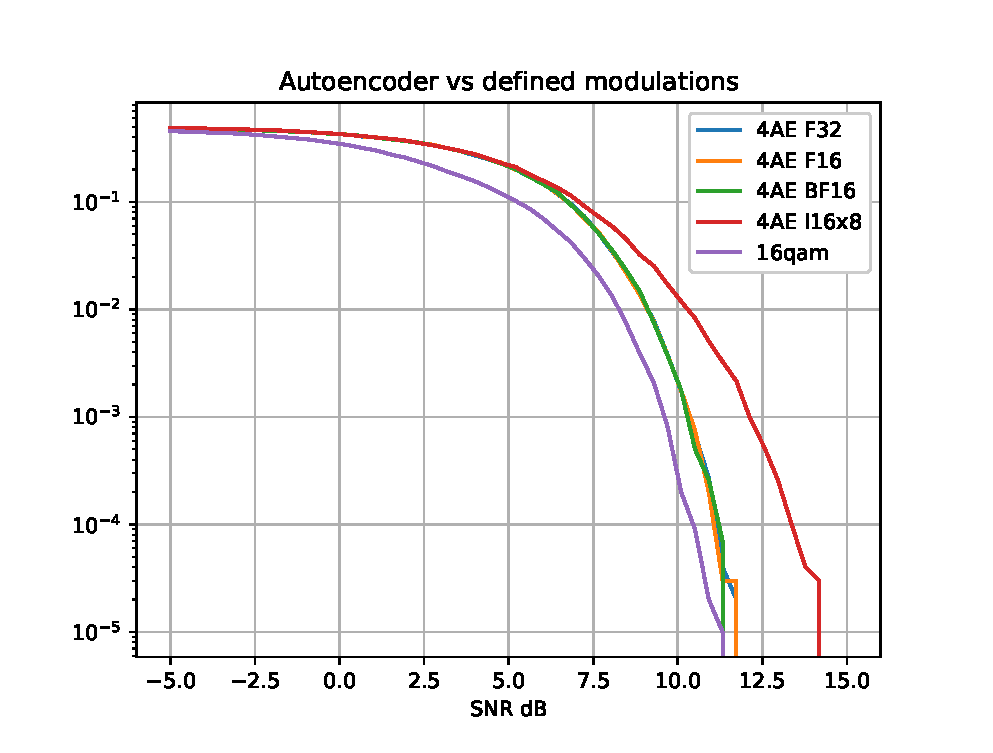
\includegraphics[width=.75\linewidth]{autoencoder_compression.eps}
        	\caption{BER/SNR graph with 4bit autoencoder (4AE) with different post-training quantisaion - 32bit and 16bit floating-point (F32 and F16); 16bit truncated floating-point (BF16) \autocite{bfloat16}; 16bit integer for activation and 8bit integer for weights (I16x8) \autocite{i16x8}}
        	\label{fig:autoenc_quant}
        \end{figure}
        
    	8bit integer test had resulted in 0.5 BER across any SNR indicating an issue with this particular data type or method. Other data types such as all 16 or 32 bit integer were not tested due to limitation in TensorFlow post-training quantization, however other techniques will be explored in the future. Results show very close accuracy between 32bit and 16bit floating-point data types indicating that 16bit FP could be used to increase training times and reduce memory and bandwidth requirements in FPGA.
    